\section{An entry-independent authority condition for gain scheduling}\label{sec:feasibility}

\citet{ozsoy2026robust} schedule $g$ over the spindle speed by maximising $\alim(\Omega,g)$ subject to an authority condition. The published form of that condition, as reproduced here, is set by the entry transient; this section replaces it by a steady-state condition in closed form, checked in the time domain with the clipped command.

\subsection{The published condition}\label{sec:feas-pub}

The published condition, Eq.~(2) of \citet{ozsoy2026robust}, simulates the cut at $a=\alim(\Omega,g)$ and accepts $g$ if the peak demand stays within the actuator rating:
\begin{equation}\label{eq:pub}
  J(g)=\begin{cases}\alim(\Omega,g) & \text{if }\max_tK_ag\lvert\dot x(t)\rvert\le F_{\max},\\[2pt] 0 & \text{otherwise,}\end{cases}
\end{equation}
with $g^\star(\Omega)=\arg\max_{g\in\mathcal G}J(g)$. The demand, written there as $g\lvert\dot x\rvert$ with $g$ in \si{\volt\second\per\metre} and compared with \SI{27}{\newton}, is read here as the force of Eq.~\eqref{eq:pub}; read as a voltage, it would make the gains 2--3 times larger. Nor is the start of the simulation stated. A step entry from rest (full engagement at $t=0$, zero history) reproduces the published gains at \SIrange{2320}{3000}{\rpm} (median ratio 0.97) and was used. Elsewhere the reproduced gains are 0.74 (500--\SI{1150}{\rpm}) and 0.88 (1160--\SI{1490}{\rpm}) times the published ones (medians outside the straight segments of the published map), 0.27--1.3 times at 1870--\SI{2050}{\rpm} and 1.2--1.9 times at 2060--\SI{2310}{\rpm} (Fig.~\ref{fig:feas}a; Supplementary Material).
% src: src/objective.py (demand K_a g max|x'|), src/gainmap.py, src/run_gain_map.py; README §2, §4.6 (start not stated; demand read as a force; voltage reading 2-3x), §5.2 (gain ratio 0.97 at 2320-3000 rpm; 0.74, 0.88 and 1.2-1.9 by speed range), §6 (voltage reading: results/gainmap_volt.npz); results/paper_vs_ours.json (p04: band medians 0.74, 0.88, 1.83, 0.97 with the straight segments of the published map excluded; band_1870_2050_range 0.27-1.3); verification/targets/fig8_gain_map.csv (published map), README §4.4 (straight segments); recomputed from gainmap_main.npz g_best and fig8_gain_map.csv: range 1.19-1.91 at 2060-2310 rpm

With this start the peak demand is set by the entry transient: at \SI{2500}{\rpm} and $g=536$ the peak per revolution falls from \SI{27}{\newton} in the first revolution to \SI{16}{\newton} in the fiftieth. The condition thus measures how strongly the entry excites the cut, not the authority needed in settled cutting, and its optimum depends on the start: with a feed ramp of one or ten revolutions, or a face entry (Section~\ref{sec:bistab-prot}), it becomes 2900--\SI{3000}{\volt\second\per\metre} at \SI{2500}{\rpm} ($\alim=38$--\SI{40}{\milli\metre}) instead of 536. As the depth moves with $g$ and the forced response oscillates in the depth [Eq.~\eqref{eq:Fm}], the demand is not monotone in $g$, and in the reproduction the feasible set fragments: at \SI{2300}{\rpm} the demand exceeds \SI{27}{\newton} above $g\approx400$ ($\alim\approx\SI{6}{\milli\metre}$) and falls below it again only in a narrow pocket near $g\approx850$ ($\alim\approx\SI{12}{\milli\metre}$). Such pockets hold the optimum throughout 2060--\SI{2310}{\rpm}, where the reproduced gains exceed the published ones, so they belong to the reproduced objective and need not occur in the computation of \citet{ozsoy2026robust}.
% src: verification/claim_audit/claim_audit.json (27.0 N in rev 0 -> 16.0 N in rev 49 at 2500 rpm, g = 536); verification/paper/support_runs.json (Eq. 2 optimum at 2500 rpm on a 50 V s/m grid: feed ramp 1 rev 2900 V s/m, 38.29 mm; 10 rev 3000, 40.03 mm; face entry 2950, 39.15 mm); README §4.6, §5.2 (pockets at all of 2060-2310 rpm; connected-interval gain 0.72 of the published), §8.1; results/gainmap_main.npz (scan_g, scan_fd, scan_alim at 2300 rpm: 27.1 N at g = 400, a_lim 5.99 mm; optimum 849.3 V s/m, a_lim 11.87 mm)

\subsection{A steady-state authority condition}\label{sec:feas-new}

The reformulated condition requires that, once the cut has settled, the command stays inside the clip at every depth the gain admits, up to a margin $\kappa<1$ below the stability limit. Below $\alim$ the settled motion is the forced orbit of Eq.~\eqref{eq:xp}, so the condition has a closed form:
\begin{equation}\label{eq:feas}
  \begin{aligned}
    F_{\mathrm{ss}}(\Omega,g)&=\max_{0<a\le\kappa\,\alim(\Omega,g)}K_a\,\bmax(a)\le F_{\max},\\
    g^\star(\Omega)&=\max\bigl\{g\in\mathcal G:\ F_{\mathrm{ss}}(\Omega,g)\le F_{\max}\bigr\},
  \end{aligned}
\end{equation}
with $\kappa=0.9$ and $\mathcal G=[0,g_{\max}]$, $g_{\max}=1500$ or \SI{3000}{\volt\second\per\metre} (the published method does not state its search interval). Each harmonic of $b$ grows with $g$ as long as $1+g\operatorname{Re}z>0$, where $z=i\omega G_a(i\omega)G(i\omega)$ at its frequency; $F_{\mathrm{ss}}$ can then fall with $g$ only through the phase alignment of the harmonics or a shrinking depth range (Supplementary Material). On a grid of gains the feasible set was one interval $[0,g_b]$ at every speed, and $g^\star=g_b$ was found by bisection. The closed form matches the simulator's settled demand to within the latter's axial quadrature error (Supplementary Material).
% src: src/feasibility.py (KAPPA = 0.9, N_DEPTH = 80, demand_envelope, edge_gain); README §8.2; harmonic condition from Eqs. (Gcl) and (xp): b_m = -F_m(a) (i w G) g/(1 + g z), z = i w Ga G (derivation in supp_s3.tex); verification/paper/feas_monotone.json (251 speeds x 151 gains: all_one_interval true); results/feas_g1500.npz (cert_demand_td vs cert_demand_cf), verification/feasibility/cf_vs_td_layers.json

The steady condition cannot see the entry. Each scheduled gain was therefore checked by step entries from rest with the clipped command and the full surface memory (Section~\ref{sec:bistab-prot}), on a ladder of depths from $0.225\alim$ in steps of \SI{8}{\percent} up to $\kappa\alim$; a ladder is needed because with saturation stability need not be monotone in the depth. The clipped limit $a_{\mathrm{TD}}(g^\star)$ found in this way defines the checked depth
\begin{equation}\label{eq:achk}
  \achk=\min\bigl\{\kappa\,\alim(g^\star),\ a_{\mathrm{TD}}(g^\star)\bigr\},
\end{equation}
which rests on the simulation of one entry and is not a certificate.
% src: src/run_feas_certify.py (a_lo = 0.25 kappa a_lim, growth 1.08, nreg = 0); src/tdboundary.py (boundary); README §8.3

\subsection{Results}\label{sec:feas-res}

The reproduced map of Eq.~\eqref{eq:pub} jumps where its optimum enters or leaves a pocket (Fig.~\ref{fig:feas}a); the reformulated map, with $\mathcal G=[0,1500]$, has no jumps. Its gain sits at this chosen bound at 157 of the 251 speeds; elsewhere (1530--\SI{2460}{\rpm}) the steady demand binds, and the gain dips to \SI{135}{\volt\second\per\metre} at \SI{1940}{\rpm}, where the tooth-passing frequency matches the natural frequency. Both maps have their minimum at this forced resonance.
% src: results/gainmap_main.npz (g_best: jumps at 2000-2010 and 2310-2320 rpm; minimum 71.1 V s/m at 1950 rpm); results/feas_g1500.npz (at_bound: 157; g_best < 1500 over 1530-2460 rpm, minimum 134.9 V s/m at 1940 rpm); README §5.2, §8.4

The entry check binds at 112 of the 251 speeds, those at which the run at the operating depth $\kappa\alim$ did not settle. Averaged over all speeds (Table~\ref{tab:feas}, Fig.~\ref{fig:feas}b), $\achk=\SI{15.87}{\milli\metre}$, at mostly larger gains, against \SI{12.75}{\milli\metre} for $\alim$ at the gains of Eq.~\eqref{eq:pub}, which carries no margin, and \SI{5.85}{\milli\metre} without control. The smallest checked depth is \SI{12.57}{\milli\metre} (\SI{2140}{\rpm}), against \SI{5.97}{\milli\metre} (\SI{2330}{\rpm}) for Eq.~\eqref{eq:pub}. Only at 1500--\SI{2050}{\rpm}, near the forced resonance, is the mean $\achk$ below the depth of Eq.~\eqref{eq:pub}. With the same clipped step entry and full memory, the time-domain limit at the nine speeds of the clipped-DVF comparison of \citet[Table~3]{ozsoy2026robust} is 6.4--\SI{12.1}{\milli\metre} at the gains of Eq.~\eqref{eq:pub} and 12.6--\SI{17.0}{\milli\metre} at those of Eq.~\eqref{eq:feas} (Supplementary Material).
% src: results/feas_cert_g1500.npz (a_lim, a_op_linear, a_td_clipped, a_cert: a_cert < a_op_linear at 112 speeds, exactly where results/feas_g1500.npz cert_stable = 0; mean 15.87 mm; minimum 12.57 mm at 2140 rpm), results/feas_g1500.npz (g_best, a_unc: mean 5.85 mm), results/gainmap_main.npz (a_best: mean 12.75 mm, minimum 5.97 mm at 2330 rpm; g_best below the reformulated gain at 239 of 251 speeds, recomputed); README §8.3, §8.4; results/table3_main.csv (a_prop_td 6.37-12.12 mm), results/feas_compare_g1500.json (table3: a_new_td 12.60-16.97 mm)

\begin{table}[!tbp]
  \centering
  \caption{Mean depths (\si{\milli\metre}) by speed range: checked depth $a_{\mathrm{chk}}$ of the reformulated condition [Eqs.~\eqref{eq:feas}--\eqref{eq:achk}, $\mathcal G=[0,1500]$, $\kappa=0.9$], $a_{\lim}$ at the gains of Eq.~\eqref{eq:pub} (no margin), and the uncontrolled limit $a_{\lim}(0)$.}
  \label{tab:feas}
  \begin{tabular}{@{}lrrrr@{}}
    \toprule
    Speeds (rpm) & Number & $a_{\mathrm{chk}}$ & $a_{\lim}$, Eq.~\eqref{eq:pub} & $a_{\lim}(0)$\\
    \midrule
    500--1150  & 66  & 16.75 & 12.36 & 4.02\\
    1160--1490 & 34  & 14.89 & 11.49 & 3.87\\
    1500--2050 & 56  & 20.51 & 21.24 & 16.58\\
    2060--3000 & 95  & 12.87 & 8.47  & 1.51\\
    All        & 251 & 15.87 & 12.75 & 5.85\\
    \bottomrule
  \end{tabular}
  \par\smallskip
  \parbox{0.9\linewidth}{\footnotesize Sensitivity (Supplementary Material): with $\kappa=0.95$ the gains change by at most \SI{0.53}{\volt\second\per\metre}; a guard of $0.85F_{\max}$ lowers the gain at 116 speeds; with $g_{\max}=3000$ the mean $\achk$ is \SI{17.1}{\milli\metre} and the entry check binds at 184 speeds.}
\end{table}
% src: results/feas_cert_g1500.npz (a_cert), results/gainmap_main.npz (a_best), results/feas_g1500.npz (a_unc); README §8.4; note: results/feas_k095.npz (gains within 0.53 V s/m), results/feas_guard085.npz (116 speeds lowered), results/feas_cert_g3000.npz (mean a_cert 17.13 mm; a_cert < a_op_linear at 184 speeds); README §8.5

The reformulated condition does not depend on the entry, but it gives up what the published one provides for a specified entry: keeping that entry inside the linear range at $a=\alim$, a conservative but meaningful requirement on its basin. The basin therefore has to be assessed separately (Sections~\ref{sec:bistability} and~\ref{sec:certificates}). The check, too, has limits: it simulates a single entry, once per depth of the ladder, and at \SI{1070}{\rpm} the ladder of Section~\ref{sec:bistab-map}, which starts from another depth, finds chatter at $0.83\alim$, below $\achk=0.90\alim$. Finally, $\achk$ lies inside the bistable band at 104 of the 109 speeds where the band was found (Section~\ref{sec:bistab-map}), so a checked depth is not a safe depth.
% src: README §8.6; results/c1_map.npz vs results/feas_cert_g1500.npz (1070 rpm: a_step_clip/a_lim = 0.831, a_cert/a_lim = 0.900); results/c1_band.npz vs results/feas_cert_g1500.npz (104/109)

\begin{figure}[!tbp]
  \centering
  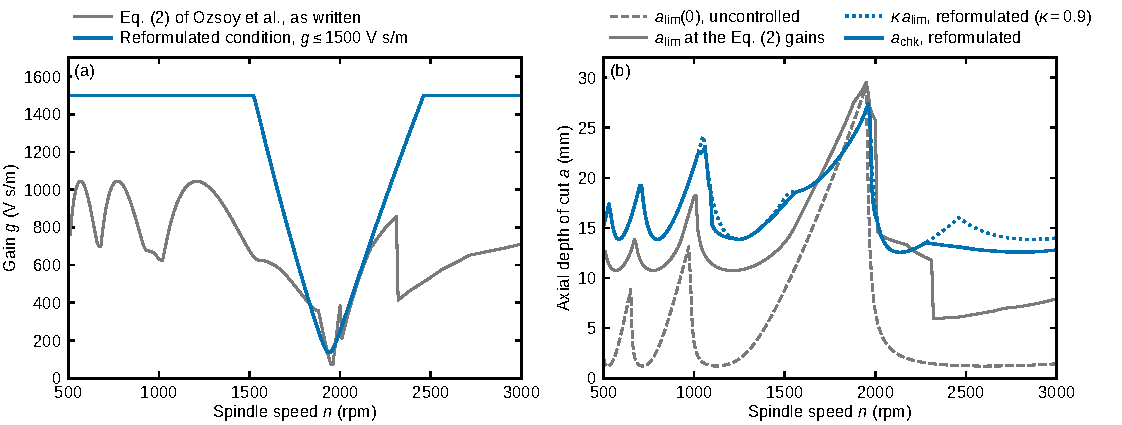
\includegraphics[width=\textwidth]{figures/fig02_feasibility.pdf}
  \caption{Gain scheduling under the two authority conditions over \SIrange{500}{3000}{\rpm}. (a)~Gain maps: the published condition, Eq.~\eqref{eq:pub}, reproduced with a step entry, the reformulated condition, Eq.~\eqref{eq:feas} with $\mathcal G=[0,1500]$, and the published map of \citet{ozsoy2026robust}. (b)~Depths: uncontrolled limit $a_{\lim}(0)$, $a_{\lim}$ at the gains of Eq.~\eqref{eq:pub}, $\kappa a_{\lim}$ and the checked depth $a_{\mathrm{chk}}$ of Eq.~\eqref{eq:achk} at the reformulated gains.}
  \label{fig:feas}
\end{figure}
